\section{Task definition}

Consider the air treatment of a blast furnace based on a centrifugal compressor (CC) driven by an induction.
Design and simulate speed control and DTC in order to cover the given fluid demand at least one decade faster than the intrinsic characteristic of the uncontrolled system.

\subsection{Known parameters}

Rated power supply parameters
\begin{itemize}
	\item Rated voltage $V_n = 380 \unit{\V}$
	\item Rated frequency $f_n = 50 \unit{\Hz}$
	\item Pole pairs $n_p = 3$
\end{itemize}

Electrical parameters
\begin{itemize}
	\item Stator resistance $R_s = 0.24 \unit{\ohm}$
	\item Stator inductance $L_s = 59.4 \unit{\mH}$
	\item Rotor resistance $R_r = 0.175 \unit{\ohm}$
	\item Rotor inductance $L_r = 59.1 \unit{\mH}$
	\item Mutual inductance $l_m = 57 \unit{\mH}$
\end{itemize}

Mechanical parameters
\begin{itemize}
	\item Motor inertia $J = 0.4 \unit{\kg\square\m}$
	\item Friction coefficient $\beta = 0.068 \unit{\N\m\s\per\radian}$
\end{itemize}

Load parameters
\begin{itemize}
	\item Gearbox ratio $r = \frac{\omega_l}{\omega_m} = 4$
	\item Torque load $T^l_l = h \omega_l^2$ where $h = 0.009 \unit{\N\m\square\s\per\square\radian}$
\end{itemize}

Process power supply parameters
\begin{itemize}
	\item Power supply voltage $V_{ac} = 230 \unit{\V}$
	\item Power supply frequency $f_{ac} = 50 \unit{\Hz}$
\end{itemize}

\subsection{Assigned task}

It is required to design a DTC control in order to deal with the assigned process speed profile shown in \autoref{fig:target-speed-profile}.

\begin{figure}[htbp]
	\centering
	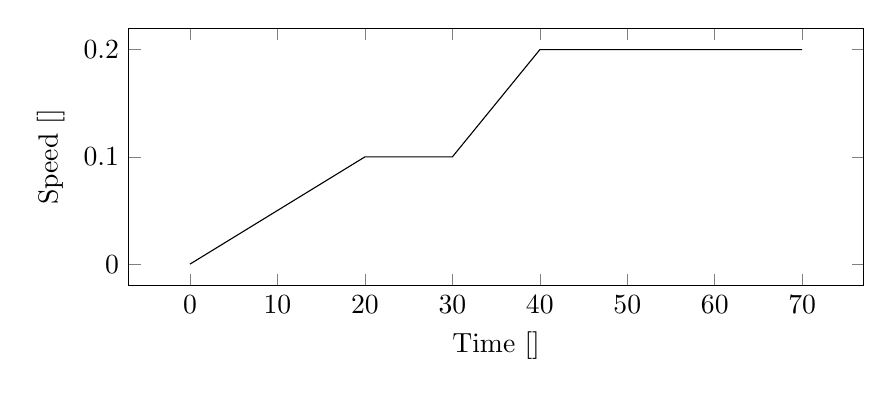
\begin{tikzpicture}
	\begin{axis}
		[
		width=0.9\textwidth,
		height=0.4\textwidth,
		xlabel={Time $[\unit{\second}]$},
		ylabel={Speed $[\unit{\percent}]$},
		xtick distance = 10,
		ytick distance = 0.1
		]
		\addplot[] coordinates {(0,0) (20,0.1) (30,0.1) (40,0.2) (70,0.2)};
	\end{axis}
	\end{tikzpicture}
	\caption{Assigned speed profile}
	\label{fig:target-speed-profile}
\end{figure}

\section{Induction motor model}

The target motor of the project is a classical three-phase squirrel cage induction.
To define a valid model of the motor, we can start from the dynamic equivalent circuit of the three-phase induction motor shown in \autoref{fig:generic-induction-motor-model}.

\begin{figure}[htb]
	\centering
	\begin{circuitikz}[american voltages]
		\draw
		(0,3) coordinate(Vs+)
		to [short, *-] ++(0.5,0)
		to [R, l=$R_s$] ++(2,0)
		to [L, l=$L_s - L_m$] ++(2,0)
		to [short, i=$\vec{i}_s$] ++(1,0) coordinate(Vm+)
		to [short, i<=$\vec{i}_r$] ++(1,0)
		to [L, l=$L_r - L_m$] ++(2,0)
		to [R, l=$R_r$] ++(2,0)
		to [short, -*] ++(0.5,0) coordinate(Vr+);
		\draw
		(0,0) coordinate(Vs-)
		to [short, *-] ++(0,0)
		to [V, v=$j\dot\theta_s\vec\Psi_s$, invert] (Vs- -| Vm+) coordinate(Vm-)
		to [V, v=$j\dot\theta_r\vec\Psi_r$] (Vs- -| Vr+)
		to [short, -*] ++(0,0) coordinate(Vr-);
		\draw
		(Vm+)
		to [L, l=$L_m$, i>^=$\vec{i}_s+\vec{i}_r$] (Vm-);
		\draw (Vs-) to [open, v=$\vec{V}_s$, voltage=straight] (Vs+);
		\draw (Vr-) to [open, v=$\vec{V}_r$, voltage=straight] (Vr+);

	\end{circuitikz}
	\caption{Generic induction motor model}
	\label{fig:generic-induction-motor-model}
\end{figure}

Due to the presence of the squirrel cage, we have to impose $\vec{V}_r=0$ and it can be demonstrated that by manipulating the model, we can get the equivalent one shown in \autoref{fig:induction-motor-squirrel-cage-generic} with $k$ arbitrary value.

\begin{figure}[htb]
	\centering
	\begin{circuitikz}[american voltages]
		\draw
		(0,3) coordinate(Vs+)
		to [short, *-] ++(0.5,0)
		to [R, l=$R_s$] ++(2,0)
		to [L, l=$L_s - k L_m$] ++(2,0)
		to [short, i=$\vec{i}_s$] ++(1,0) coordinate(Vm+)
		to [short, i<=$\vec{i}'_r$] ++(1,0)
		to [L, l=$k^2 L_r - k L_m$] ++(2,0)
		to [R, l=$k^2 R_r$] ++(2,0)
		to [short, -] ++(0.5,0) coordinate(Vr+);
		\draw
		(0,0) coordinate(Vs-)
		to [short, *-] ++(0,0)
		to [V, v=$j\dot\theta_s\vec\Psi_s$, invert] (Vs- -| Vm+) coordinate(Vm-)
		to [V, v=$j\dot\theta_r\vec\Psi_r$] (Vs- -| Vr+)
		to [short, -] ++(0,0) coordinate(Vr-);
		\draw
		(Vm+)
		to [L, l=$k L_m$, i>^=$\vec{i}_s+\vec{i}'_r$] (Vm-);
		\draw (Vs-) to [open, v=$\vec{V}_s$, voltage=straight] (Vs+);
		\draw (Vr-) -- (Vr+);

	\end{circuitikz}
	\caption{Generic induction motor model}
	\label{fig:induction-motor-squirrel-cage-generic}
\end{figure}

Choosing $k=L_m/L_r$ we got the four-parameters model shown in \autoref{fig:induction-motor-four-parameters} where the rotor inductance disappears, where:

\begin{align*}
	L_{ks} &= L_s-\frac{L_m^2}{L_r} \\
	L_{km} &= \frac{L_m^2}{L_r} \\
	R_{kr} &= R_r\frac{L_m}{L_r}
\end{align*}

\begin{figure}[htb]
	\centering
	\begin{circuitikz}[american voltages]
		\draw
		(0,3) coordinate(Vs+)
		to [short, *-] ++(0.5,0)
		to [R, l=$R_s$] ++(2,0)
		to [L, l=$L_{ks}$] ++(2,0)
		to [short, i=$\vec{i}_s$] ++(1,0) coordinate(Vm+)
		to [short, i<=$\vec{i}'_r$] ++(1,0)
		to [R, l=$R_{kr}$] ++(2,0)
		to [short, -] ++(0.5,0) coordinate(Vr+);
		\draw
		(0,0) coordinate(Vs-)
		to [short, *-] ++(0,0)
		to [V, v=$j\dot\theta_s\vec\Psi_s$, invert] (Vs- -| Vm+) coordinate(Vm-)
		to [V, v=$j\dot\theta_r\vec\Psi_r$] (Vs- -| Vr+)
		to [short, -] ++(0,0) coordinate(Vr-);
		\draw
		(Vm+)
		to [L, l=$L_{km}$, i>^=$\vec{i}_s+\vec{i}'_r$] (Vm-);
		\draw (Vs-) to [open, v=$\vec{V}_s$, voltage=straight] (Vs+);
		\draw (Vr-) -- (Vr+);

	\end{circuitikz}
	\caption{Four parameters induction motor model}
	\label{fig:induction-motor-four-parameters}
\end{figure}

The model in \autoref{fig:induction-motor-four-parameters} is described by the \autoref{eq:four-parameters-model}.

\begin{align}
	\label{eq:four-parameters-model}
	\vec{V}_s &= R_s \vec{i}_s + p \vec\Psi_s + j \dot\theta_s\vec\Psi_s \nonumber \\
	0 &= R_{kr} \vec{i}'_r + p \vec\Psi_r + j \dot\theta_r\vec\Psi_r \nonumber \\
	\vec\Psi_s &= L_{ks}\vec{i}_s + \vec\Psi_r \nonumber \\
	\vec\Psi_r &= L_{km} (\vec{i}_s + \vec{i}'_r)
\end{align}

\small{Where $p$ indicates time derivative ($\frac{d}{dt}$)}

Choosing a \textbf{stationary} reference frame ($\alpha\beta$) fixed on the stator, we have $\dot\theta_s = 0$ and $\dot\theta_r = - \omega_r$; the final model is shown in \autoref{fig:four-parameters-stationary} and \autoref{eq:four-parameters-model-fixed-frame}.

\begin{figure}[htb]
	\centering
	\begin{circuitikz}[american voltages]
		\draw
		(0,3) coordinate(Vs+)
		to [short, *-] ++(0.5,0)
		to [R, l=$R_s$] ++(2,0)
		to [L, l=$L_{ks}$] ++(2,0)
		to [short, i=$\vec{i}_{s_{\alpha\beta}}$] ++(1,0) coordinate(Vm+)
		to [short, i<=$\vec{i}'_{r_{\alpha\beta}}$] ++(1,0)
		to [R, l=$R_{kr}$] ++(2,0)
		to [short, -] ++(0.5,0) coordinate(Vr+);
		\draw
		(0,0) coordinate(Vs-)
		to [short, *-] (Vs- -| Vm+) coordinate(Vm-)
		to [V, v=$-j\omega_r\vec\Psi_{r_{\alpha\beta}}$] (Vs- -| Vr+)
		to [short, -] ++(0,0) coordinate(Vr-);
		\draw
		(Vm+)
		to [L, l=$L_{km}$, i>^=$\vec{i}_{s_{\alpha\beta}}+\vec{i}'_{r_{\alpha\beta}}$] (Vm-);
		\draw (Vs-) to [open, v=$\vec{V}_{s_{\alpha\beta}}$, voltage=straight, voltage shift=1pt] (Vs+);
		\draw (Vr-) -- (Vr+);
	\end{circuitikz}
	\caption{Four parameters model with stationary reference frame}
	\label{fig:four-parameters-stationary}
\end{figure}

\begin{align}
	\label{eq:four-parameters-model-fixed-frame}
	\vec{V}_{s_{\alpha\beta}} &= R_s \vec{i}_{s_{\alpha\beta}} + p \vec\Psi_{s_{\alpha\beta}} \nonumber \\
	0 &= R_{kr} \vec{i}'_{r_{\alpha\beta}} + p \vec\Psi_{r_{\alpha\beta}} - j \omega_r\vec\Psi_{r_{\alpha\beta}} \nonumber \\
	\vec\Psi_{s_{\alpha\beta}} &= L_{ks}\vec{i}_{s_{\alpha\beta}} + \vec\Psi_{r_{\alpha\beta}} \nonumber \\
	\vec\Psi_{r_{\alpha\beta}} &= L_{km} (\vec{i}_{s_{\alpha\beta}} + \vec{i}'_{r_{\alpha\beta}}) \nonumber \\
	T_e &= n_p \Im(\vec{i}_{s_{\alpha\beta}}\undervec\Psi_{s_{\alpha\beta}})
\end{align}

The Simulink implementation of the electrical model is shown in \autoref{fig:simulink-inductor-motor-electrical-part}.

\begin{figure}[htb]
	\centering
	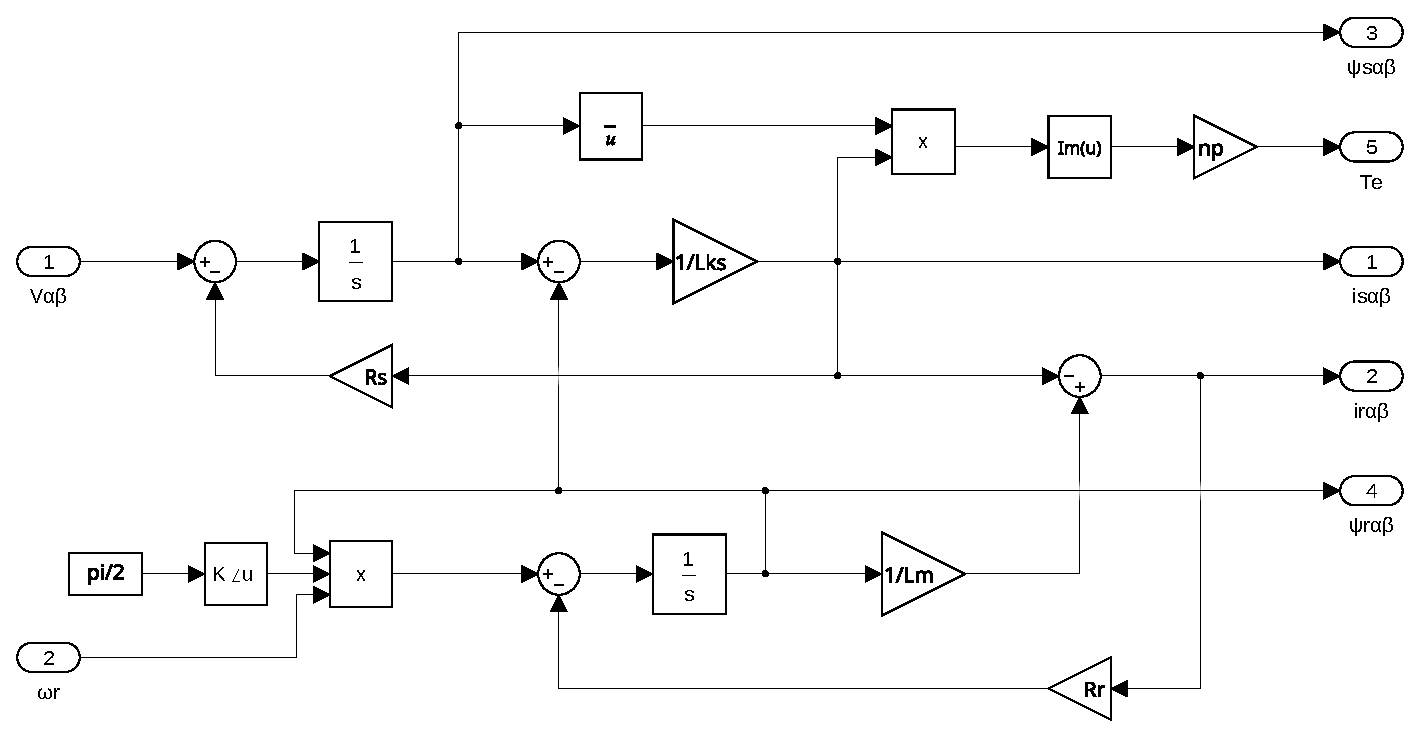
\includegraphics[width=\textwidth]{schematics/inductor_motor_electrical_part}
	\caption{Electrical part of four-parameters induction motor Simulink schematic}
	\label{fig:simulink-inductor-motor-electrical-part}
\end{figure}

Mechanical part described by \autoref{eq:model-mechanical-part} completed the model as shown \autoref{fig:simulink-inductor-motor}.

\begin{align}
	\label{eq:model-mechanical-part}
	J \dot\omega_m + \beta\omega_m &= T_e - T_l \nonumber \\
	\omega_r &= n_p \omega_m
\end{align}

The model exposes also the fluxes ($\vec{\Psi}_{s_{\alpha\beta}}$, $\vec{\Psi}_{r_{\alpha\beta}}$), rotor current ($\vec{i}'_{r_{\alpha\beta}}$) and torque ($T_e$) which in a real scenario are not directly measurable; these should be estimated exploiting current and voltage stator measurements.

\begin{figure}[htb]
	\centering
	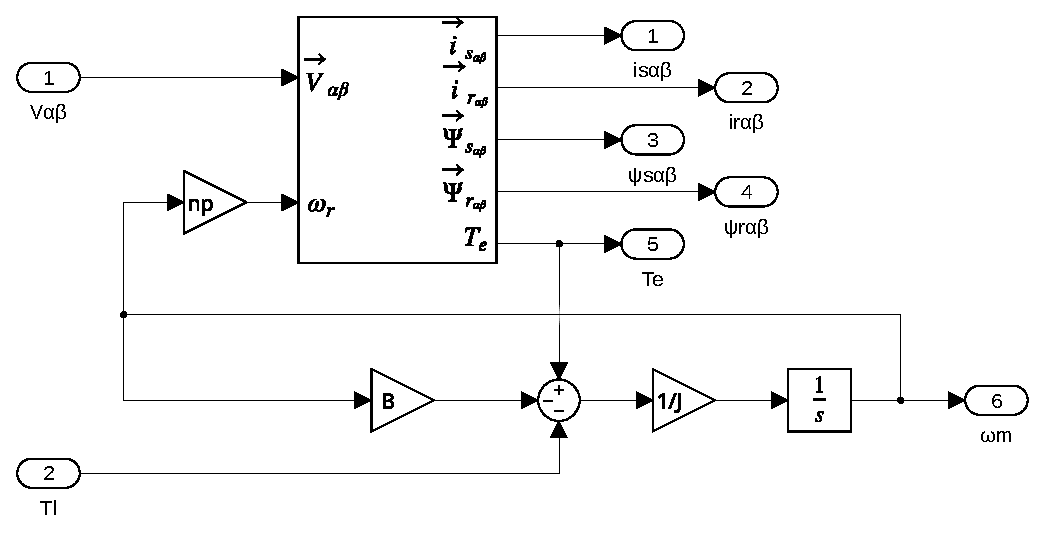
\includegraphics[width=\textwidth]{schematics/inductor_motor}
	\caption{Completed four-parameters induction motor Simulink schematic}
	\label{fig:simulink-inductor-motor}
\end{figure}

\subsection{Fixed reference frame transformation}\label{subsec:stationary-reference-frame-transformation}

Three-phase quantities in order to be used in the fixed space phasor reference frame ($\alpha\beta$) have to be converted in a space phasor quantity with \autoref{eq:to-fixed-space-phasor}; the scale factor $\sqrt{2/3}$ guaranteed that in the case of consider quantity is balanced three-phase voltage source, the module of the phasor is equal to the RMS value of the line voltage.
That transformation was implemented in simulink as shown in \autoref{fig:simulink-to-fixed-space-phasor}.

\begin{equation}
	\vec{X}_{\alpha\beta} = \sqrt{\frac{2}{3}}\left( X_a + X_b e^{\j\frac{2}{3}\pi} + X_c e^{-\j\frac{2}{3}\pi}\right)
	\label{eq:to-fixed-space-phasor}
\end{equation}

\begin{figure}[htb]
	\centering
	\subfloat[\centering Block]{{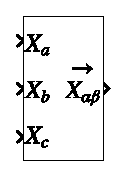
\includegraphics[width=0.11\textwidth]{schematics/to_fixed_space_phasor_block} }}
	\qquad
	\subfloat[\centering Implemetation]{{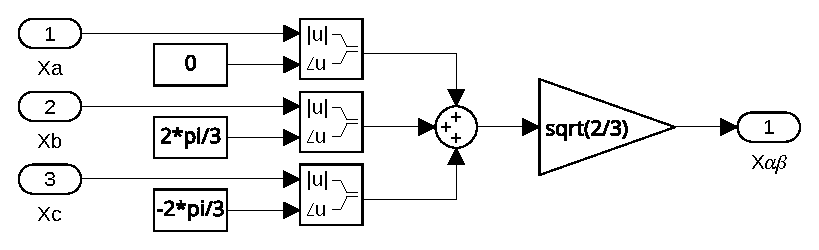
\includegraphics[width=0.6\textwidth]{schematics/to_fixed_space_phasor} }}
	\caption{To fixed space phasor transformation Simulink schematic}
	\label{fig:simulink-to-fixed-space-phasor}
\end{figure}

\subsection{Load model}

The inductor motor is connected with the load through a gear box.
The ideal gear box model is shown in \autoref{eq:ideal-gear-box}, where $T^l_l$ is the torque load seen from the load.

\begin{align}
	\omega_l &= r \omega_m \nonumber \\
	T^l_l &= \frac{1}{r} T_l
	\label{eq:ideal-gear-box}
\end{align}

So, seen from the motor, the load has the form of \autoref{eq:load}.

\begin{equation}
	T_l = h r^3 \omega_m^2
	\label{eq:load}
\end{equation}

\section{Finding missing parameters}

To find some useful motor parameters, we can set some tests on the model using the provided parameters.

\subsection{No-load test}

In the no-load test the motor is powered with rated voltage without any load (\autoref{fig:simulink-no-load-test}).

\begin{figure}[htb]
	\centering
	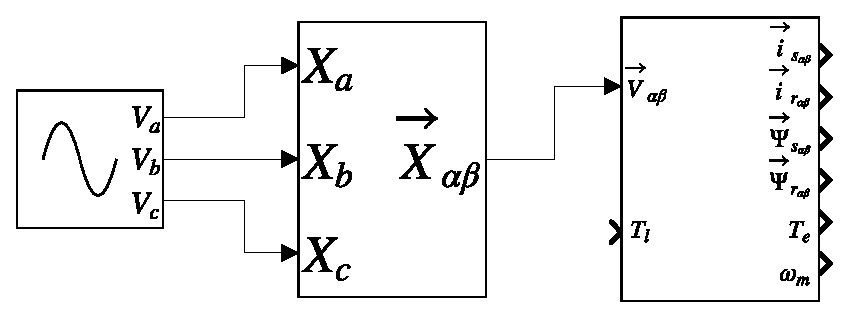
\includegraphics[width=0.7\textwidth]{schematics/no_load_test}
	\caption{Simulink no load test schematic}
	\label{fig:simulink-no-load-test}
\end{figure}

Looking at stator flux evolution (\autoref{fig:no-load-stator-flux}) we can see it reach an equilibrium value of about $\qty{1.48}{\weber}$, we can consider this value as the flux stator rated value $\Psi_{s_n}$.
We can assume $\Psi_{s_n}$ is a good working point, indeed, using stator flux values less or near this value guarantees the good exploits of ferromagnetic characteristic reducing the no linear effect of inductances (\autoref{fig:typical-current-vs-flux}).

\begin{figure}[htb]
	\centering
	\begin{tikzpicture}[declare function={
	Psisn = 1.48;
	}]
		\begin{axis}
			[
			xlabel={Time $[\unit{\s}]$},
			ylabel={Stator flux magnitude $[\unit{\weber}]$},
			xmin=0, xmax=0.6,
			ymin=0, ymax=2.5,
			ytick distance=1,
			extra y ticks={Psisn},
			extra y tick labels={$\Psi_{s_n}$}
			]

			\addplot[]
			table[
			x=t,
			y expr=sqrt((\thisrow{Psis_a})^2 + (\thisrow{Psis_b})^2)
			] {data/no_load_test-stator_flux.csv};

			\addplot[dashed, color=lightgray] {Psisn};
		\end{axis}
	\end{tikzpicture}
	\caption{No load test: Stator flux}
	\label{fig:no-load-stator-flux}
\end{figure}

\begin{figure}[htbp]
	\centering
	\begin{tikzpicture}
		\begin{axis}
			[
			xlabel={Current $[\unit{\A}]$},
			ylabel={Flux $[\unit{\weber}]$},
			ymin=0, ymax=1.1,
			xtick=\empty,
			ytick={0.9},
			yticklabels={$\Psi_n$}
			]
			\addplot[domain=0:10] {(2/(1+exp(-0.8*x)))-1};
			\addplot[domain=0:10, dashed, color=lightgray] {0.9};
		\end{axis}
	\end{tikzpicture}
	\caption{Typical characteristic current vs. flux in ferromagnetic circuit}
	\label{fig:typical-current-vs-flux}
\end{figure}

\subsection{Torque vs. speed curve}

To compute torque speed relation, the model used until now is not suitable.
Let's consider model \autoref{fig:induction-motor-squirrel-cage-generic} again, if we chose $k=L_s/L_m$ we are able to make disappear the stator inductance (\autoref{fig:four-parameters-stationary-no-stator-inductance}).

\begin{figure}[htb]
	\centering
	\begin{circuitikz}[american voltages]
		\draw
		(0,3) coordinate(Vs+)
		to [short, *-] ++(0.5,0)
		to [R, l=$R_s$] ++(2,0)
		to [short, i=$\vec{i}_{s_{\alpha\beta}}$] ++(1,0) coordinate(Vm+)
		to [short, i<=$\vec{i}'_{r_{\alpha\beta}}$] ++(1,0)
		to [L, l=$L_{kr}$] ++(2,0)
		to [R, l=$R'_{kr}$] ++(2,0)
		to [short, -] ++(0.5,0) coordinate(Vr+);
		\draw
		(0,0) coordinate(Vs-)
		to [short, *-] (Vs- -| Vm+) coordinate(Vm-)
		to [V, v=$-j\omega_r\vec\Psi_{r_{\alpha\beta}}$] (Vs- -| Vr+)
		to [short, -] ++(0,0) coordinate(Vr-);
		\draw
		(Vm+)
		to [L, l=$L'_{km}$, i>^=$\vec{i}_{s_{\alpha\beta}}+\vec{i}'_{r_{\alpha\beta}}$] (Vm-);
		\draw (Vs-) to [open, v=$\vec{V}_{s_{\alpha\beta}}$, voltage=straight, voltage shift=1pt] (Vs+);
		\draw (Vr-) -- (Vr+);
	\end{circuitikz}
	\caption{Alternative four-parameters model with stationary reference frame}
	\label{fig:four-parameters-stationary-no-stator-inductance}
\end{figure}

Introducing the concept of \textbf{slip} with \autoref{eq:slip} where $\omega$ is the frequency of the power voltage source and considering the system at steady state, it can be shown that the model can be re-written with \autoref{eq:rotor-resistance-slip} gotten \autoref{fig:four-parameters-stationary-no-stator-inductance-slip}.

\begin{equation}
	x = \frac{\omega - \omega_r}{\omega}\
	\label{eq:slip}
\end{equation}

\begin{equation}
	-j\omega_r\vec\Psi_{r_{\alpha\beta}} = \frac{1-x}{x}R'_{kr}
	\label{eq:rotor-resistance-slip}
\end{equation}

\begin{figure}[htb]
	\centering
	\begin{circuitikz}[american voltages]
		\draw
		(0,3) coordinate(Vs+)
		to [short, *-] ++(0.5,0)
		to [R, l=$R_s$] ++(2,0)
		to [short, i=$\vec{i}_{s_{\alpha\beta}}$] ++(1,0) coordinate(Vm+)
		to [short, i<=$\vec{i}'_{r_{\alpha\beta}}$] ++(1,0)
		to [L, l=$L_{kr}$] ++(2,0)
		to [R, l=$R'_{kr}$] ++(2,0)
		to [short, -] ++(0,0) coordinate(Vr+);
		\draw
		(0,0) coordinate(Vs-)
		to [short, *-] (Vs- -| Vm+) coordinate(Vm-)
		to [short, -] (Vs- -| Vr+) coordinate(Vr-);
		\draw
		(Vm+)
		to [L, l=$L'_{km}$, i>^=$\vec{i}_{s_{\alpha\beta}}+\vec{i}'_{r_{\alpha\beta}}$] (Vm-);
		\draw (Vs-) to [open, v=$\vec{V}_{s_{\alpha\beta}}$, voltage=straight, voltage shift=1pt] (Vs+);
		\draw (Vr-) to [R, l=$R'_{kr}\frac{1-x}{x}$] (Vr+);
	\end{circuitikz}
	\caption{Model at steady state}
	\label{fig:four-parameters-stationary-no-stator-inductance-slip}
\end{figure}

Due to the small voltage drop on $R_s$, we can move it on the rotor side accepting a small approximation (\autoref{fig:four-parameters-approximation-stator-resistance-stator-side}); this makes the stator voltage drop equal to the common inductance one, allowing us to compute a simple relation between torque and motor speed shown in \autoref{eq:torque-steady-state}.

\begin{figure}[htb]
	\centering
	\begin{circuitikz}[american voltages]
		\draw
		(0,3) coordinate(Vs+)
		to [short, i=$\vec{i}_{s_{\alpha\beta}}$, *-] ++(1,0) coordinate(Vm+)
		to [short, i<=$\vec{i}'_{r_{\alpha\beta}}$] ++(1,0)
		to [R, l=$R_s$] ++(2,0)
		to [L, l=$L_{kr}$] ++(2,0)
		to [R, l=$R'_{kr}$] ++(2,0)
		to [short, -] ++(0,0) coordinate(Vr+);
		\draw
		(0,0) coordinate(Vs-)
		to [short, *-] (Vs- -| Vm+) coordinate(Vm-)
		to [short, -] (Vs- -| Vr+) coordinate(Vr-);
		\draw
		(Vm+)
		to [L, l=$L'_{km}$, i>^=$\vec{i}_{s_{\alpha\beta}}+\vec{i}'_{r_{\alpha\beta}}$] (Vm-);
		\draw (Vs-) to [open, v=$\vec{V}_{s_{\alpha\beta}}$, voltage=straight, voltage shift=1pt] (Vs+);
		\draw (Vr-) to [R, l=$R'_{kr}\frac{1-x}{x}$] (Vr+);
	\end{circuitikz}
	\caption{Approximation model with stator resistance moved to rotor side}
	\label{fig:four-parameters-approximation-stator-resistance-stator-side}
\end{figure}

\begin{equation}
	\overline{T}_e = 3 \frac{R'_{kr}}{x} \frac{n_p}{\omega} \frac{V_{s_{\alpha\beta}}^2}{\left(R_s + \frac{R'_{kr}}{x}\right)^2 + \omega^2 L_{kr}^2}
	\label{eq:torque-steady-state}
\end{equation}

The torque-speed curve at rated values is shown in \autoref{fig:torque-vs-speed}; from this chart we can found some useful values such as the starting torque $T_{e_{st}}\approx\qty{465}{\newton\meter}$ and the maximum torque $T_{e_{max}}\approx\qty{1762}{\newton\meter}$

The sector defined by the speed at maximum torque and base speed is called stable region (when the torque load increases the motor decreases its speed to compensate).
The rated motor speed $\omega_n$ lies in this region.

\begin{figure}[htbp]
	\centering
	\begin{tikzpicture}[declare function={
		Rs		= 0.24;
		Rr		= 0.175;
		Ls		= 0.0594;
		Lr		= 0.0591;
		Lm		= 0.057;
		k		= Ls / Lm;
		Rkr		= Rr * k^2;
		Lkr		= Lr * k^2 - Lm * k;
		Vsn		= sqrt(3/2) * 380;
		wn		= 50 * 2 * pi;
		np		= 3;
		wb		= wn / np;
		Te(\x)		= 3 * (Rkr / \x) * (np / wn) * Vsn^2 / ( (Rs + (Rkr / \x))^2 + (wn * Lkr)^2 );
		slip(\wm)	= (wb - \wm) / wb;
		xmax		= Rkr / sqrt(Rs^2 + (wn*Lkr)^2);
		wmax		= wb(1-xmax);
		Tmax		= Te(xmax);
		Tstart		= Te(1);
	}]
	\begin{axis}
		[
		xlabel={Motor speed $[\unit{\rad\per\second}]$},
		ylabel={Torque $[\unit{\N\m}]$},
		xtick distance = 30,
		ytick distance = 750,
		extra x ticks={wb},
		extra x tick labels={$\omega_b$},
		extra y ticks={Tmax, Tstart},
		extra y tick labels={$T_{e_{max}}$, $T_{e_{st}}$}
		]
		\addplot[
			domain=0:wb),
			samples=300
		] {Te(slip(x))};

		\addplot[domain=0:1.1*wb, dashed, lightgray] {Tmax};
		\addplot[domain=0:1.1*wb, dashed, lightgray] {Tstart};
	\end{axis}
	\end{tikzpicture}
	\caption{Torque vs speed at rated condictions}
	\label{fig:torque-vs-speed}
\end{figure}

\subsection{Uncontrolled system response}\label{subsec:uncontrolled-system-response}

We have to estimate the time response of the system in order to deal with the requirement of a system on a decade faster than the uncontrolled one.

In the \autoref{fig:simulink-uncontrolled-response-test} is shown the simulink schematic of the uncontrolled system.

\begin{figure}[htb]
	\centering
	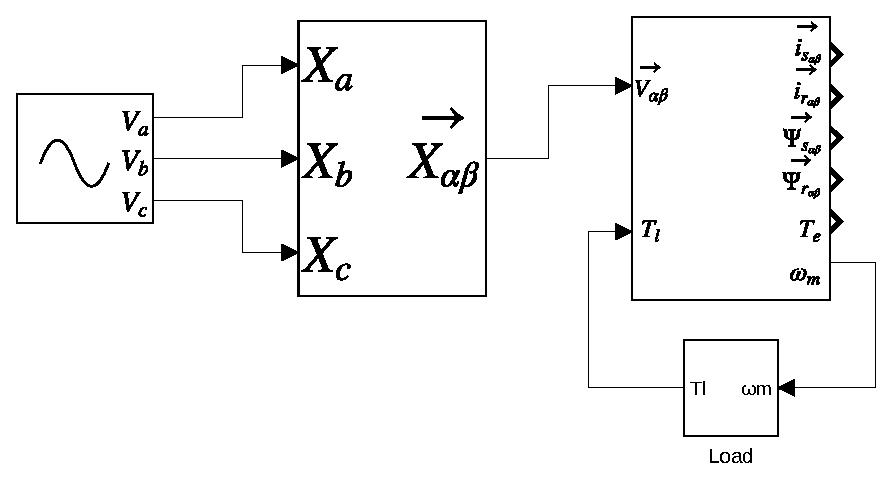
\includegraphics[width=0.7\textwidth]{schematics/uncontrolled_response}
	\caption{Simulink uncontrolled system schematic}
	\label{fig:simulink-uncontrolled-response-test}
\end{figure}

The system is putting in the working condition, and its response to the reference step is recorded. The evolution of the speed is shown in \autoref{fig:uncontrolled-response}.
From it, we can extrapolate the time assessment (i.e., time necessary to the response to reach and remain in the $\qty{1}{\percent}$ neighborhood of the steady state value), which is bound with the intrinsic speed characteristic of the system by a constant of about $4\div5$.
We can estimate $T_{a1\%} \approx \qty{1.236}{\second}$.

\begin{figure}[htbp]
	\centering
	\begin{tikzpicture}[declare function={
		wf=55.29;
		wt=wf*0.99;
		Tu=1.236;
	}]
		\begin{axis}
			[
			width=0.9\textwidth,
			height=0.4\textwidth,
			xlabel={Time $[\unit{\second}]$},
			ylabel={Motor speed $[\unit{\radian\per\second}]$},
			xtick distance=0.5,
			extra x ticks={Tu},
			extra x tick labels={$T_{a1\%}$},
			extra y ticks={wt},
			extra y tick labels={$\qty{99}{\percent}\omega_{m_\infty}$},
			]
			\addplot[blue] table[
			x=t,
			y=wm
			] {data/uncontrolled_response.csv};

			\draw[dashed, lightgray]
			({rel axis cs:0,0}|-{axis cs:0,wt}) -- ({axis cs:0,wt}-|{rel axis cs:1,1});

			\draw[dashed, lightgray]
			(axis cs:Tu,0) -- ({axis cs:Tu,0}|-{axis cs:0,wt});
		\end{axis}
	\end{tikzpicture}
	\caption{Uncontrolled motor response in speed}
	\label{fig:uncontrolled-response}
\end{figure}

\section{Power suply}

The DTC approach involves operating with three-phase VSI fed by a Direct Current source.

\subsection{Voltage rectifier}

Considering a three-phase balanced AC power source, this has to be rectified before it can be used to feed the VSI.
To perform this operation, it can be used a three-phase diode bridge rectifier (\autoref{fig:voltage-rectifier-circuit}); this guaranteed a nearly constant voltage output of $\sqrt{3}V_f$ with a disturbance at six times the AC frequency.

\begin{figure}[htb]
	\centering
	\begin{circuitikz}[american voltages]
		\draw (0,-2) -- (0,2);
		\foreach \Y/\f in {2/a,0/b,-2/c} {
			\draw
			(0,\Y)
			to [V, v=$V_\f$, isourcesin] ++(2,0)
			to [L] ++(2,0);
		}
		\foreach \X in {0,1.5,3} {
			\draw
			(5, 0) ++ (\X,-2.5)
			to [diode] ++(0,1.5)
			to [short] ++(0,2)
			to [diode] ++(0,1.5);
		}
		\draw (4,0) to [short,-*] ++ (2.5,0);
		\draw (4,2) -- ++(0,-1) to [short,-*] ++(1,0);
		\draw (4,-2) -- ++(0,1) to [short,-*] ++(4,0);
		\draw (9.5,-2.5) to [C] ++(0,5);
		\draw (5,0) ++(0,2.5) to [short, -*] ++(6,0) node (A) {};
		\draw (5,0) ++(0,-2.5) to [short, -*] ++(6,0) node (B) {};
		\draw (B) to [open, v=$V_{dc}$, voltage=straight] (A);
	\end{circuitikz}
	\caption{Three-phase diode bridge rectifier circuit schematic}
	\label{fig:voltage-rectifier-circuit}
\end{figure}

To reduce the simulation complexity and considering the minor entity of the noise, we will consider the rectifier ideal, and we will use in the simulation a constant DC voltage source.

\subsection{Voltage Source Inverter}

The VSI powered with a DC voltage source allows modulating the three-phase signal with three PWM signals.
The simplest circuit schematic is composed of six transistors with bulk diode as shown in \autoref{fig:vsi-circuit}.

\begin{figure}[htb]
	\centering
	\begin{circuitikz}[american voltages]
		\draw (0,2.5) node (A) {} to [short, *-] ++(6,0);
		\draw (0,-2.5) node (B) {} to [short, *-] ++(6,0);
		\draw (B) to [open, v=$V_{dc}$, voltage=straight] (A);

		\foreach \X/\f in {0/a,2/b,4/c} {
			\draw
			(2, 0) ++ (\X,-2.5)
			to [Tnpn, bodydiode, n=l] ++(0,2)
			-- ++(0,1)
			to [Tnpn, bodydiode, n=h] ++(0,2);
			\draw (h.G) node ()[anchor=south] {$S_\f$};
			\draw (l.G) node ()[anchor=south] {$\bar{S}_\f$};
		}
		\foreach \X/\Y/\f in {0/0.75/a,2/0/b,4/-0.75/c} {
			\draw (2,0) ++(\X,\Y) to [short, *-*] (8,\Y) node ()[anchor=south east] {$V_\f$};
		}

	\end{circuitikz}
	\caption{Voltage Source Inverter circuit schematic}
	\label{fig:vsi-circuit}
\end{figure}

For the simulation scenario the transistors are considered ideal as shown in \autoref{fig:simulink-vsi-schematic}.

\begin{figure}[h!]
	\centering
	\subfloat[\centering Block]{{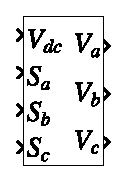
\includegraphics[width=0.15\textwidth]{schematics/vsi_block} }}
	\qquad
	\subfloat[\centering Implemetation]{{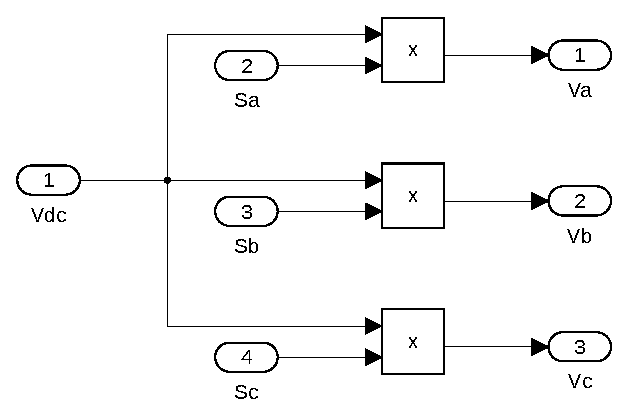
\includegraphics[width=0.4\textwidth]{schematics/vsi} }}
	\caption{Voltage Source Inverter Simulink schematic}
	\label{fig:simulink-vsi-schematic}
\end{figure}

\section{Direct Torque Control}

\subsection{Switching table}

The main component of DTC is the switching table.

It expects the following inputs:
\begin{itemize}
	\item[$\tau$] It can assume three values: $1$, $0$ and $-1$ respectively, the torque has to be increased (to CCW direction), the torque has to not change, the torque has to decrease(to CW direction).
	\item[$\phi$] It can assume three values: $1$ and $0$ respectively, the flux magnitude has to decrease or increase.
	\item[$\theta(N)$] It can assume integer values in range \numrange{1}{6} indicating in with sector stator flux lies.
\end{itemize}

This information is responsible for providing the voltage phases status used to drive the VSI exploiting the switching table, which implementation is shown in \autoref{lst:lstlisting}.

\begin{lstlisting}[language=matlab,label={lst:lstlisting},caption=Switching table implemetation]
function [sa,sb,sc] = fcn(tau,phi,thetaN)

phi = ((phi > 0.5) * 1) + 1;
tau = ((tau > 0.5) * 1 + (tau < -0.5) * -1) + 2;

% T(phi+1, tau+2, thetaN, V)
T = zeros(2,3,6,3);

T(1,3,1,:) = [0 1 0];
T(1,2,1,:) = [0 0 0];
T(1,1,1,:) = [0 0 1];
T(2,3,1,:) = [1 1 0];
T(2,2,1,:) = [1 1 1];
T(2,1,1,:) = [1 0 1];

T(1,3,2,:) = [0 1 1];
T(1,2,2,:) = [1 1 1];
T(1,1,2,:) = [1 0 1];
T(2,3,2,:) = [0 1 0];
T(2,2,2,:) = [0 0 0];
T(2,1,2,:) = [1 0 0];

T(1,3,3,:) = [0 0 1];
T(1,2,3,:) = [0 0 0];
T(1,1,3,:) = [1 0 0];
T(2,3,3,:) = [0 1 1];
T(2,2,3,:) = [1 1 1];
T(2,1,3,:) = [1 1 0];

T(1,3,4,:) = [1 0 1];
T(1,2,4,:) = [1 1 1];
T(1,1,4,:) = [1 1 0];
T(2,3,4,:) = [0 0 1];
T(2,2,4,:) = [0 0 0];
T(2,1,4,:) = [0 1 0];

T(1,3,5,:) = [1 0 0];
T(1,2,5,:) = [0 0 0];
T(1,1,5,:) = [0 1 0];
T(2,3,5,:) = [1 0 1];
T(2,2,5,:) = [1 1 1];
T(2,1,5,:) = [0 1 1];

T(1,3,6,:) = [1 1 0];
T(1,2,6,:) = [1 1 1];
T(1,1,6,:) = [0 1 1];
T(2,3,6,:) = [1 0 0];
T(2,2,6,:) = [0 0 0];
T(2,1,6,:) = [0 0 1];

S = squeeze(T(phi, tau, thetaN,:));

sa = S(1);
sb = S(2);
sc = S(3);
\end{lstlisting}

In a real scenario, reinitialising the switching table at each step is an anti-pattern; this is imposed by the Matlab function block limitations, which does not allow you to define persistent constants between multiple iterations, anyway due to the simulation scenario, this behavior is not a real issue.

\subsection{Stator flux sector computation}

The stator flux sector computation is performed exploiting a matlab function shown in \autoref{fig:simulink-dtc-flux-sector-schematic}.

\begin{figure}[h!]
	\centering
	\begin{subfigure}{.2\textwidth}
		\centering
		\begin{minipage}{.1cm}
			\vfill
		\end{minipage}
		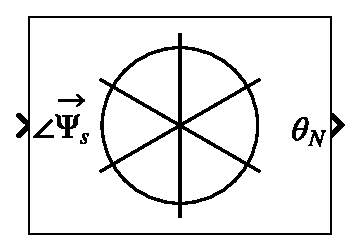
\includegraphics[width=0.8\textwidth]{schematics/sector_compute_block}
		\begin{minipage}{.1cm}
			\vfill
		\end{minipage}
		\caption{Block}
	\end{subfigure}
	\qquad
	\begin{subfigure}{.7\textwidth}
		\begin{lstlisting}[language=matlab]
function thetaN = fcn(theta)

sector_number = 6;
sector_size = 2*pi / sector_number;
first_sector_offset = sector_size /2;

% move first sector start from -first_sector_offset to 0
theta = theta + first_sector_offset;

theta = rem(theta, 2*pi);

% make theta always positive
theta = theta + (theta < 0) * 2*pi;

thetaN = floor(theta /sector_size) + 1;

% prevent overflow due to numerical errors
thetaN = thetaN - (thetaN > sector_number) * sector_number;
		\end{lstlisting}
		\caption{Implemetation}
	\end{subfigure}
	\caption{DTC stator flux sector computation}
	\label{fig:simulink-dtc-flux-sector-schematic}
\end{figure}

\subsection{Stator flux magnitude control}

The computation of the variable $\phi$ is based on a hysteresis function driven by stator flux magnitude error $e_{\Psi_s}$ (\autoref{fig:simulink-dtc-flux-threashold-schematic}).
This hysteresis function exposes one degree of freedom ($\Delta \Psi$) with which you can balance the allowed error $e_{\Psi_s}$ and the frequency switching of the VSI.

\begin{figure}[h!]
	\centering
	\subfloat[\centering Block]{{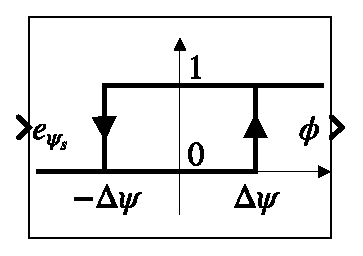
\includegraphics[width=0.3\textwidth]{schematics/flux_threashold_block} }}
	\qquad
	\subfloat[\centering Implemetation]{{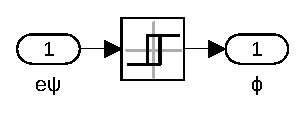
\includegraphics[width=0.4\textwidth]{schematics/flux_threshold} }}
	\caption{DTC stator flux threashold schematic}
	\label{fig:simulink-dtc-flux-threashold-schematic}
\end{figure}

\subsubsection{Choosing \texorpdfstring{$\Delta \Psi$}{dPsi}}\label{subsubsec:choosing-delta-psi}

To find a good value of $\Delta\Psi$ we set up a simulation with no load and the $\tau$ variable fix to $1$ as shown in \autoref{fig:simulink-flux-tuning}.

\begin{figure}[htbp]
	\centering
	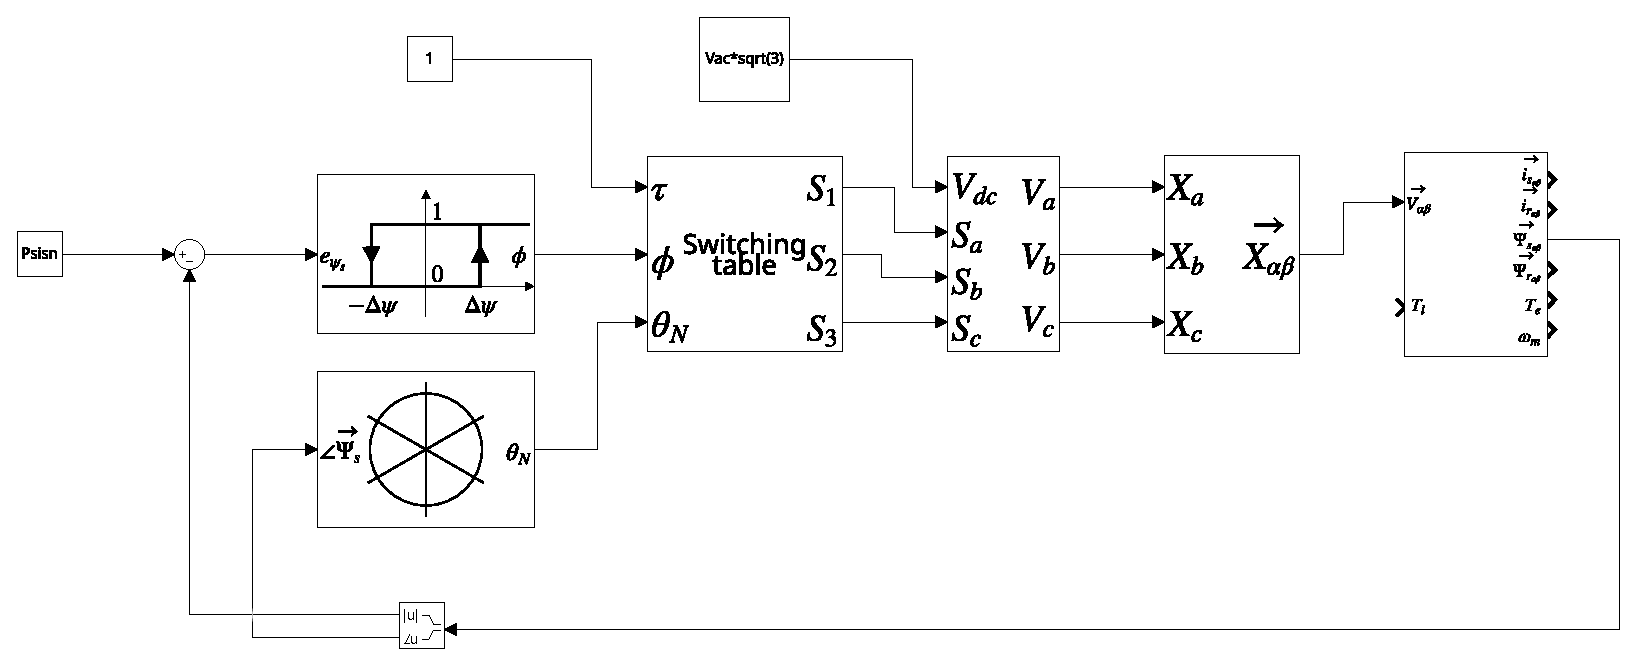
\includegraphics[width=0.8\textwidth]{schematics/flux_tuning}
	\caption{Flux tuning schematic}
	\label{fig:simulink-flux-tuning}
\end{figure}

The simulation was repeated for different value of $\Delta\Psi$ while the switching frequency of $\phi$ is monitored.
The results of the simulations are shown in \autoref{fig:flux-switching-frequency-comparison}.

\begin{nb}
	Directly monitoring $\phi$ permits to decouple switching frequency from the sector computation effect, but it is important to note that maximum switching allowed has to be referred to the single phase on the VSI.
\end{nb}

\begin{figure}[htbp]
	\centering
	\begin{tikzpicture}
		\begin{axis}
			[
			width=0.9\textwidth,
			height=0.5\textwidth,
			xlabel={Time},
			ylabel={$\phi$ switching frequency $[\unit{\Hz}]$},
			xmax=0.34,
			ymin=500,
			xtick=\empty,
			ymode=log
			]

			\addplot table[
			x=t,
			y=f_01
			] {data/flux_tuning-switching_frequency.csv};
			\addlegendentry{$\Delta \Psi = 0.1\%\Psi_{s_n}$}

			\addplot table[
			x=t,
			y=f_02
			] {data/flux_tuning-switching_frequency.csv};
			\addlegendentry{$\Delta \Psi = 0.2\%\Psi_{s_n}$}

			\addplot table[
			x=t,
			y=f_05
			] {data/flux_tuning-switching_frequency.csv};
			\addlegendentry{$\Delta \Psi = 0.5\%\Psi_{s_n}$}

			\addplot table[
			x=t,
			y=f_1
			] {data/flux_tuning-switching_frequency.csv};
			\addlegendentry{$\Delta \Psi = 1\%\Psi_{s_n}$}

			\addplot table[
			x=t,
			y=f_2
			] {data/flux_tuning-switching_frequency.csv};
			\addlegendentry{$\Delta \Psi = 2\%\Psi_{s_n}$}

			\addplot table[
			x=t,
			y=f_5
			] {data/flux_tuning-switching_frequency.csv};
			\addlegendentry{$\Delta \Psi = 5\%\Psi_{s_n}$}
		\end{axis}
	\end{tikzpicture}
	\caption{Flux switching frequency for differents $\Delta \Psi$ values}
	\label{fig:flux-switching-frequency-comparison}
\end{figure}

In \autoref{fig:controlled-stator-flux-5pc}, we can see that the circular trajectory of rotor flux is guaranteed also for $\vec{\Psi}_{s_{\alpha\beta}}$ with $\Delta\Psi=5\%\Psi_{s_n}$.

\begin{figure}[htbp]
	\centering
	\begin{tikzpicture}[declare function={
		Psisn =		1.48;
		dPsi =		0.05 * Psisn;
		Psismin =	Psisn - dPsi;
		Psismax =	Psisn + dPsi;
	}]
		\begin{polaraxis}
		[
			y axis line style={draw=none},
			ymax=1.8,
			xtick={30, 90, ..., 330},
			ytick={Psismin, Psismax},
			yticklabel=\empty
		]
			\addplot[
				data cs=cart,
				color=blue,
				decoration={
					markings,
					mark=between positions 0.1 and 0.9 step 0.2 with {\arrow{stealth}}
				},
				postaction=decorate
			]
			table[
			x=Psis_a,
			y=Psis_b
			] {data/flux_tuning-5pc.csv};
			\addlegendentry{$\vec{\Psi}_{s_{\alpha\beta}}$}


			\addplot[
				data cs=cart,
				color=red,
				decoration={
					markings,
					mark=between positions 0.1 and 0.9 step 0.2 with {\arrow{stealth}}
				},
				postaction=decorate
			]
			table[
			col sep=comma,
			x=Psir_a,
			y=Psir_b
			] {data/flux_tuning-5pc.csv};
			\addlegendentry{$\vec{\Psi}_{r_{\alpha\beta}}$}

		\end{polaraxis}
	\end{tikzpicture}
	\caption{Controlled stator flux with $\Delta\Psi=5\%\Psi_{s_n}$}
	\label{fig:controlled-stator-flux-5pc}
\end{figure}

\subsection{Torque control}

To can control (and limit) the switching frequency of these discrete states the torque error drives the control variable through two hysteresis functions as shown in \autoref{fig:simulink-dtc-torque-threashold-schematic}.
The control exposes one degree of freedom ($\Delta T$), high $\Delta T$ value involves slow pursuit of the reference torque, low value involves high VSI switching rate.

\begin{figure}[h!]
	\centering
	\subfloat[\centering Block]{{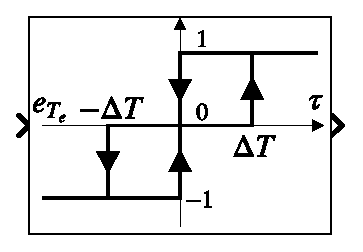
\includegraphics[width=0.3\textwidth]{schematics/torque_threashold_block} }}
	\qquad
	\subfloat[\centering Implemetation]{{\includegraphics[width=0.5\textwidth]{schematics/torque_threashold} }}
	\caption{DTC torque threashold schematic}
	\label{fig:simulink-dtc-torque-threashold-schematic}
\end{figure}

\subsubsection{Choosing \texorpdfstring{$\Delta T$}{dT}}\label{subsubsec:choosing-delta-t}

To determinate a good value for $\Delta T$ it was set a test.
With no load the system is subjected a step on the torque reference as shown in \autoref{fig:simulink-torque-tuning}, during the raising of the torque, we can check the frequency switching on the control variable $\tau$ in function of $\Delta T$.

\begin{figure}[htbp]
	\centering
	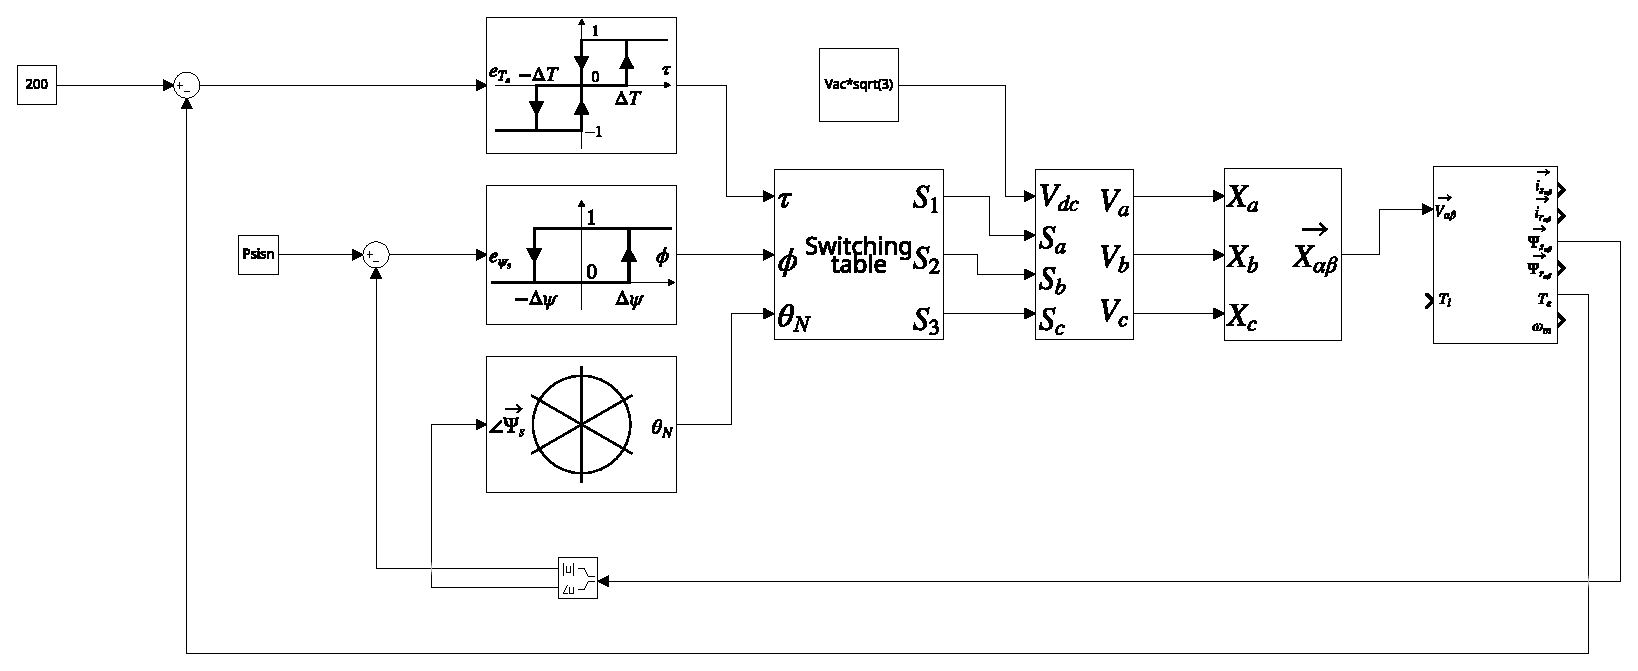
\includegraphics[width=0.8\textwidth]{schematics/torque_tuning}
	\caption{Torque tuning schematic}
	\label{fig:simulink-torque-tuning}
\end{figure}

In \autoref{fig:torque-switching-frequency-comparison} is shown the switching frequency for different values of $\Delta T$.

\begin{nb}
	As for the $\Delta \Psi$ tuning, monitoring $\tau$ instead of VSI switch phases is necessary to decouple switching frequency from the sector computation effect and flux control one.
\end{nb}

\begin{figure}[htbp]
	\centering
	\begin{tikzpicture}
		\begin{axis}
		[
			width=0.9\textwidth,
			height=0.5\textwidth,
			xlabel={Time},
			ylabel={Switching frequency $[\unit{\Hz}]$},
			xmax=0.22,
			ymin=500,
			xtick=\empty,
			ymode=log
		]

			\addplot table[
			x=t,
			y=f_05
			] {data/torque_tuning-switching_frequency.csv};
			\addlegendentry{$\Delta T = \qty{0.5}{\N\m}$}

			\addplot table[
			x=t,
			y=f_1
			] {data/torque_tuning-switching_frequency.csv};
			\addlegendentry{$\Delta T = \qty{1}{\N\m}$}

			\addplot table[
			x=t,
			y=f_2
			] {data/torque_tuning-switching_frequency.csv};
			\addlegendentry{$\Delta T = \qty{2}{\N\m}$}

			\addplot table[
			x=t,
			y=f_5
			] {data/torque_tuning-switching_frequency.csv};
			\addlegendentry{$\Delta T = \qty{5}{\N\m}$}

			\addplot table[
			x=t,
			y=f_10
			] {data/torque_tuning-switching_frequency.csv};
			\addlegendentry{$\Delta T = \qty{10}{\N\m}$}

			\addplot table[
			x=t,
			y=f_20
			] {data/torque_tuning-switching_frequency.csv};
			\addlegendentry{$\Delta T = \qty{20}{\N\m}$}

			\addplot table[
			x=t,
			y=f_50
			] {data/torque_tuning-switching_frequency.csv};
			\addlegendentry{$\Delta T = \qty{50}{\N\m}$}

		\end{axis}
	\end{tikzpicture}
	\caption{Torque switching frequency for differents $\Delta T$ values}
	\label{fig:torque-switching-frequency-comparison}
\end{figure}

\subsection{Stator flux and torque estimator}

The DTC required the measure of the stator flux and the torque, both these measures cannot make directly, so an estimator of these quantities is required.
For this purpose a V-I estimator can be used; it is described by \autoref{eq:estimator}.

\begin{align}
	\hat{\vec\Psi}_{s_{\alpha\beta}} &= \int_0^t \vec{V}_{s_{\alpha\beta}}(\tau) - R_s \vec{i}_{s_{\alpha\beta}}(\tau) d\tau \nonumber \\
	\hat{T}_e &= \Im\left( \vec{i}_{s_{\alpha\beta}} \hat{\undervec\Psi}_{s_{\alpha\beta}} \right)
	\label{eq:estimator}
\end{align}

The estimator V-I (\autoref{fig:simulink-estimator-schematic}) requires the measure of voltage and current, both these measures can be performed putting current and voltage sensors between the VSI and the motor.
For the purpose of the simulation, the dynamics of sensors are not designed, considering them ideal.
Additionally, the pure integrator is replaced with a low-pass filter to reduce the estimation error at low speed.

\begin{figure}[h!]
	\centering
	\subfloat[\centering Block]{{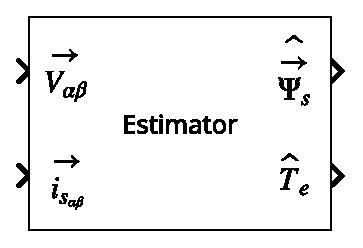
\includegraphics[width=0.15\textwidth]{schematics/estimator_block} }}
	\qquad
	\subfloat[\centering Implemetation]{{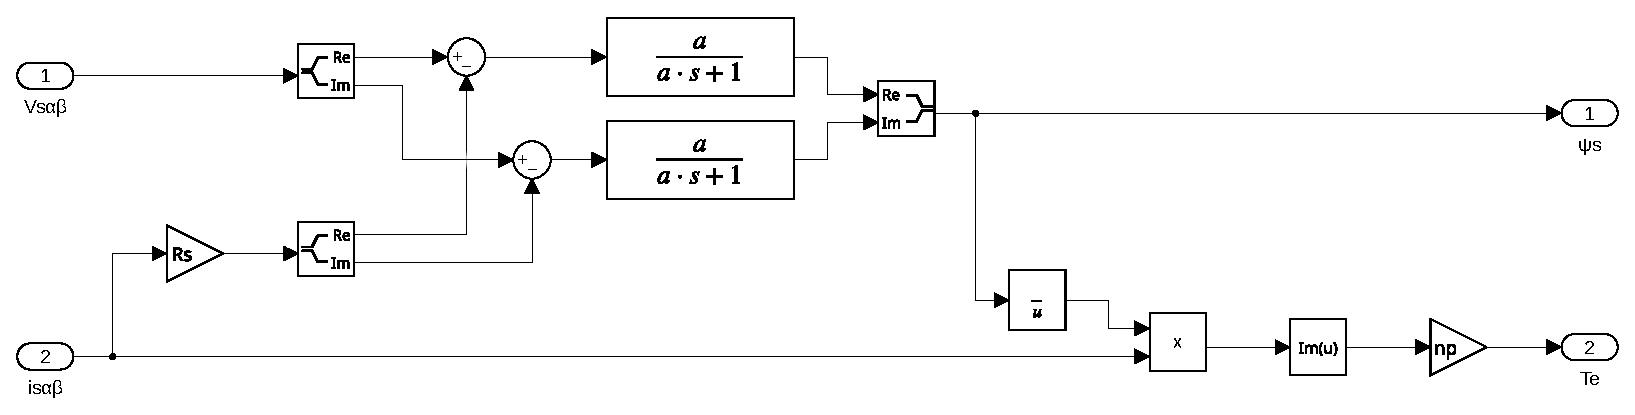
\includegraphics[width=0.75\textwidth]{schematics/estimator} }}
	\caption{Stator flux and torque estimator}
	\label{fig:simulink-estimator-schematic}
\end{figure}

\section{Speed control}

Once the inner loop of DTC has been designed, the ones on stator flux reference and speed can be realized.

\subsection{Stator flux reference loop}

From the \autoref{eq:four-parameters-model-fixed-frame}, we can deduce the approximated relation between stator voltage and flux variation shown in \autoref{eq:approximate-stator-flux-change} neglecting the typical low-voltage drop on stator resistance.

\begin{equation}
	\vec{V}_{s_{\alpha\beta}} \approx p \vec\Psi_{s_{\alpha\beta}}
	\label{eq:approximate-stator-flux-change}
\end{equation}

It is clear that if the voltage stator is limited (in our case by the available power supply voltage) then the variation speed of stator flux is also limited.
Fixed the stator flux magnitude, its rotation speed cannot grow indiscriminately; this upper limit defines the base speed of the motor ($\omega_b$) (considering the factor scale $n_p$).

To increase the motor speed beyond the base speed, we have to reduce the magnitude of stator flux at the rate of $\nicefrac{1}{\omega_m}$ to reduce the length of the ideal circular trajectory.

So the stator flux magnitude reference can be set at the nominal value as long as $\omega_m<\omega_b$, then it has to be reduced with the increase of $\omega_m$ for $\omega_m>\omega_b$ (the field weakening region).
The trend of stator flux magnitude reference is shown in \autoref{fig:flux-reference-vs-motor-speed}.

\begin{figure}[htbp]
	\centering
	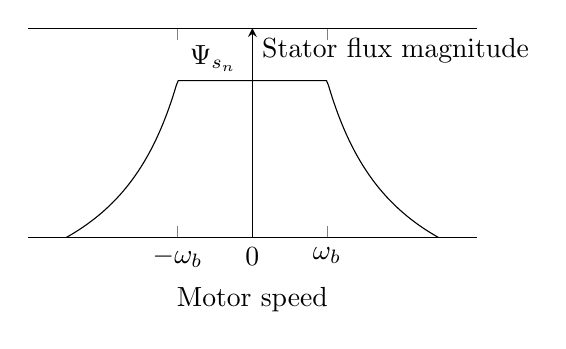
\begin{tikzpicture}[declare function={
	wb =	2;
	psin =	1;
	}]
		\begin{axis}
			[
			width=0.6\textwidth,
			height=0.35\textwidth,
			axis y line=center,
			yticklabel style={yshift=8pt},
			xlabel={Motor speed},
			ylabel={Stator flux magnitude},
			xtick={-wb,0,wb},
			xticklabels={$-\omega_b$, $0$, $\omega_b$},
			ytick={psin},
			yticklabels={$\Psi_{s_{n}}$},
			ymax=1.2*psin,
			xmin=-3*wb,
			xmax=3*wb
			]

			\addplot[samples=200] {(abs(x)<wb) * (psin) + (abs(x)>=wb) * (wb * psin / abs(x))};
		\end{axis}
	\end{tikzpicture}
	\caption{Stator flux trend in relation with motor speed}
	\label{fig:flux-reference-vs-motor-speed}
\end{figure}

Anyway, for the assigned task the motor has to operate only in the flux constant region, so this component was not included in the final control schema, replaced by a constant source at nominal value.

\subsection{Motor speed closed loop}

To regulate the motor speed, a loop has to be closed on the torque.
As regulator, we used a PI with an anti-windup system.
The speed loop requires the measurement of the motor speed ($\omega_m$), this one can be obtained exploiting an encoder put on the motor shaft; for the purpose of the simulation, the encoder dynamics was not implemented.

The complete simulink schematic is shown in \autoref{fig:simulink-completed-schematic}.

\begin{figure}[htbp]
	\centering
	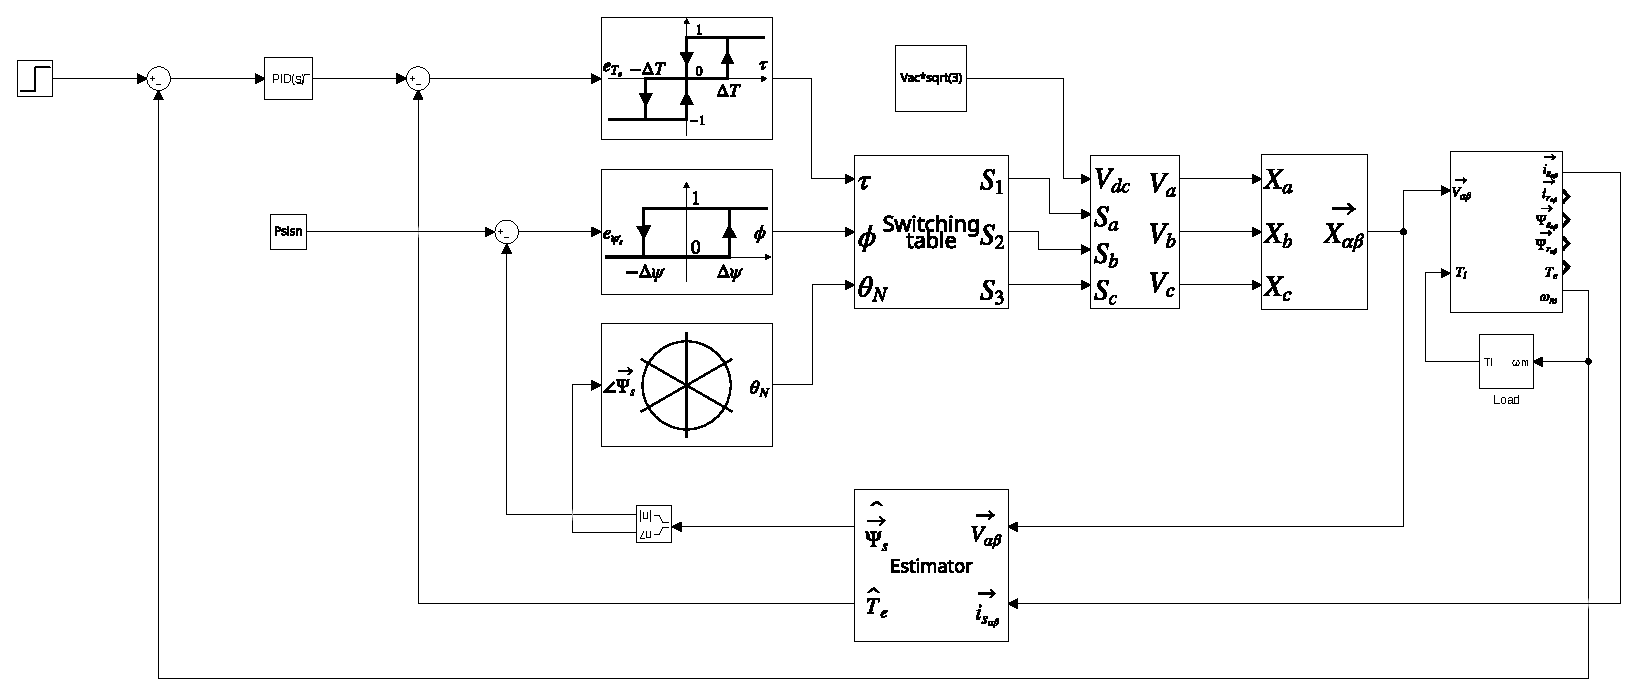
\includegraphics[width=0.9\textwidth]{schematics/completed}
	\caption{Completed schematic}
	\label{fig:simulink-completed-schematic}
\end{figure}

\subsubsection{PI tuning}

Due to the presence of the inner loop driven by hysteresis components which work on digital status, PI auto-tuning techniques (e.g.,\ Ziegler and Nichols method) are not exploitable.
Anyway, some considerations of these techniques can be used.

Setting the integral parameter to $0$ the proportional is raised as long as the $\tau$ variable starts to oscillate between $1$ and $-1$ in response to a step reference; a value below this one can be used as proportional value in the PI.

Before looking for a good value of integral action, we have to set up the anti-windup system.
Due to the strong dependency of torque by the motor speed, a unique limit in torque range cannot be found; but exploiting some simulation near the working region, we can see that the controlled motor reaches a maximum of about $\qty{380}{\N\m}$.

A good value of integral should drive the error to zero at the steady state without introducing low-frequency oscillations.

\section{Controlled system}

Following the considerations proposed in the sections above, for the assigned task we set the following parameters:
\begin{align*}
	\text{DTC} & \\
	\Delta \Psi &= \qty{2.96}{\milli\weber} \approx 0.2\%\Psi_{s_n} \\
	\Delta T &= \qty{5}{\N\m} \\
	& \\
	\text{Motor speed PI} & \\
	K_p &= 180 \\
	K_i &= 5000 \\
	T_{e_{ref}} &\in [-380,380] \\
	& \\
	\text{V-I estimator} & \\
	\text{filter time constant} &= 2
\end{align*}

\subsection{Response speed}

The project specifications require that the controller system has a response at least one decade faster than the intrinsic speed characteristic of the uncontrolled system.

In \autoref{fig:response-speed-comparison} are shown the response of the uncontrolled system (as seen in \autoref{subsec:uncontrolled-system-response}) and the controlled one.
From it, we can estimate the time assessment of the controlled system with $T^c_{a1\%}\approx\qty{0.105}{s}$.
The specification requires $\nicefrac{T^u_{a1\%}}{T^c_{a1\%}} > 10$.

\begin{equation*}
	\frac{T^u_{a1\%}}{T^c_{a1\%}} \approx 11.77 > 10
\end{equation*}

\begin{figure}[htbp]
	\centering
	\begin{tikzpicture}[declare function={
	wf = 55.29;
	wt = wf*0.99;
	Tu = 1.236;
	Tc = 0.105;
	}]
		\begin{axis}
			[
			width=0.9\textwidth,
			height=0.4\textwidth,
			xlabel={Time $[\unit{\second}]$},
			ylabel={Motor speed $[\unit{\radian\per\second}]$},
			legend style={
				legend pos=south east,
			},
			xtick distance=0.5,
			extra x ticks={Tc, Tu},
			extra x tick labels={$T^c_{a1\%}$, $T^u_{a1\%}$},
			extra y ticks={wt},
			extra y tick labels={$\qty{99}{\percent}\omega_{m_\infty}$},
			]
			\addplot[blue] table[
			x=t,
			y=wm
			] {data/uncontrolled_response.csv};
			\addlegendentry{uncontrolled system}

			\addplot[red] table[
			x=t,
			y=wm
			] {data/controlled_response.csv};
			\addlegendentry{controlled system}

			\draw[dashed, lightgray]
			({rel axis cs:0,0}|-{axis cs:0,wt}) -- ({axis cs:0,wt}-|{rel axis cs:1,1});

			\draw[dashed, lightgray]
			(axis cs:Tu,0) -- ({axis cs:Tu,0}|-{axis cs:0,wt});
			\draw[dashed, lightgray]
			(axis cs:Tc,0) -- ({axis cs:Tc,0}|-{axis cs:0,wt});
		\end{axis}
	\end{tikzpicture}
	\caption{Motor speed step response for controlled and uncontrolled systems}
	\label{fig:response-speed-comparison}
\end{figure}

\subsection{Assigned task}

In \autoref{fig:assigned-task-speed} is shown how the system motor speed follows the reference.

\begin{figure}[htbp]
	\centering
	\begin{tikzpicture}
		\begin{axis}
			[
			width=0.9\textwidth,
			height=0.4\textwidth,
			xlabel={Time $[\unit{\second}]$},
			ylabel={Rotational speed $[\unit{\radian\per\second}]$},
			legend style={
				legend pos=south east,
			}
			]

			\addplot[solid, black, semithick] table[
			x=t,
			y=wm
			] {data/assigned_task.csv};
			\addlegendentry{$\omega_{m}$}

			\addplot[dashed, red] table[
			x=t,
			y=wm_ref
			] {data/assigned_task.csv};
			\addlegendentry{$\omega_{m_{ref}}$}
		\end{axis}
	\end{tikzpicture}
	\caption{Motor speed compared to reference}
	\label{fig:assigned-task-speed}
\end{figure}

Looking at the switching frequency on a VSI phase (\autoref{fig:assigned-task-switching-frequency}), we can confirm the estimations done in \autoref{subsubsec:choosing-delta-psi} and \autoref{subsubsec:choosing-delta-t}.
On the phase A of the VSI we can see an upper limit of about $\qty{25}{\kilo\Hz}$; so a VSI with a rated frequency of $\qty{50}{\kilo\Hz}$ should be suitable for the task.
VSI can reach this kind of switching frequency also if it is based on IGBT technology.

\begin{figure}[htbp]
	\centering
	\begin{tikzpicture}
		\begin{axis}
			[
			width=0.9\textwidth,
			height=0.4\textwidth,
			xlabel={Time $[\unit{\second}]$},
			ylabel={Switching frequency $[\unit{\kilo\Hz}]$},
			y filter/.code=
				{\pgfmathdivide{#1}{1000}}
			]

			\addplot[] table[
			x=t,
			y=f_Sa
			] {data/assigned_task.csv};
		\end{axis}
	\end{tikzpicture}
	\caption{Switching frequency VSI phase A}
	\label{fig:assigned-task-switching-frequency}
\end{figure}

In \autoref{fig:assigned-task-current-fluxes} is possible to see that the current and the flux magnitudes follow the same trend (as shown also in \autoref{eq:four-parameters-model-fixed-frame}); the current grows until the stator flux magnitude reaches the steady state than is maintained rather constant (by the flux regulator of the DTC).

\begin{figure}[htbp]
	\centering
	\begin{tikzpicture}
		\begin{axis}
			[
			width=0.9\textwidth,
			height=0.4\textwidth,
			xlabel={Time $[\unit{\second}]$},
			ylabel={Current $[\unit{\ampere}]$}
			]

			\addplot[] table[
			x=t,
			y expr=sqrt((\thisrow{Is_a})^2 + (\thisrow{Is_b})^2)
			] {data/assigned_task.csv};
		\end{axis}

		\begin{axis}
			[
			width=0.9\textwidth,
			height=0.4\textwidth,
			xlabel={Time $[\unit{\second}]$},
			ylabel={Flux intensity $[\unit{\weber}]$},
			axis y line=right,
			legend style={
				legend pos=south east,
			}
			]

			\addlegendimage{black}
			\addlegendentry{$I_s$}

			\addplot[blue] table[
			x=t,
			y expr=sqrt((\thisrow{Psis_a})^2 + (\thisrow{Psis_b})^2)
			] {data/assigned_task.csv};
			\addlegendentry{$\Psi_s$}

			\addplot[red] table[
			x=t,
			y expr=sqrt((\thisrow{Psir_a})^2 + (\thisrow{Psir_b})^2)
			] {data/assigned_task.csv};
			\addlegendentry{$\Psi_r$}
		\end{axis}
	\end{tikzpicture}
	\caption{Current and fluxes magnitude (in phasor space)}
	\label{fig:assigned-task-current-fluxes}
\end{figure}

In conclusion, in \autoref{fig:assigned-task-torque} are shown the motor torque and the load one.

\begin{figure}[htbp]
	\centering
	\begin{tikzpicture}
		\begin{axis}
			[
			width=0.9\textwidth,
			height=0.4\textwidth,
			xlabel={Time $[\unit{\second}]$},
			ylabel={Torque $[\unit{\N\m}]$},
			ytick distance=5,
			legend style={
				legend pos=south east,
			}
			]

			\addplot[] table[
			x=t,
			y=Te
			] {data/assigned_task.csv};
			\addlegendentry{$T_e$}

			\addplot[red] table[
			x=t,
			y=Tl
			] {data/assigned_task.csv};
			\addlegendentry{$T_l$}
		\end{axis}
	\end{tikzpicture}
	\caption{Motor and load torques}
	\label{fig:assigned-task-torque}
\end{figure}

\section{Possible improvements}

Following some consideration about possible improvements for the proposed model.

\subsection{Models improvements}

\begin{itemize}
	\item All the measurements required in the control loops are retrieved directly from the simulated values, but in a real scenario these kinds of data have to be measured exploiting sensors.
	In order to improve the quality of the simulation, it should be modeled the dynamics of these sensors (e.g.,\ quantization, delay, stochastic error, etc.\ldots).

	\item The whole model of the controller was designed in the time continuous domain, it being about a controller that has to be digitalized, a redesign in the discrete domain with particular care about digital systems (taking into account the time quantization, computation frequency) could noticeably improve the reliability of the control simulation.

	\item Power supply and VSI dynamics have been omitted from the model in order to reduce the complexity of the simulation.
	Defined the commercial VSI, which will be used, its dynamics can be included in the model.
\end{itemize}

\subsection{Control improvements}

\begin{itemize}
	\item The DTC is heavily based on the hybrid system theory (i.e.,\ control theory where systems are modeled and regulated by a combination of state machines and differential equations).
	Regulation in this field with a traditional control system (e.g.,\ PID) involves dealing with several compromises.
	A possible improvement in control of the speed could consist in replacing the PI controller with some advanced control technique based also on the hybrid system theory (e.g.,\ switching control or MPC).
\end{itemize}
